\section{Software Design}
\phantomsection
\subsection{UML Modeling}

In this chapter are specified and documented the artifacts of Finduber system using UML diagrams. UML can be described as a general purpose visual modeling language to visualize, construct, specify and document software system. The diagrams are aim to help developers, business users and anybody interested to understand the system. To model a system the most important aspect is to capture the dynamic behaviour. There are five diagrams in UML available to model it: use case, sequence, state and activity diagram. However, class and deployment diagram are also important to examine. They represent physical and conceptual elements of the system that are present in Finduber platform as nodes and classes.

\subsection{Use Case Diagram}

Use case diagrams are used to gather the requirements of the Finduber system including internal and external agets known as actors. There is only one actor -- user -- that interacts with the system. The system functionalities are captured in use cases as shown in the Figure \ref{usecase_uml}.

\begin{figure}[!ht]
\centering
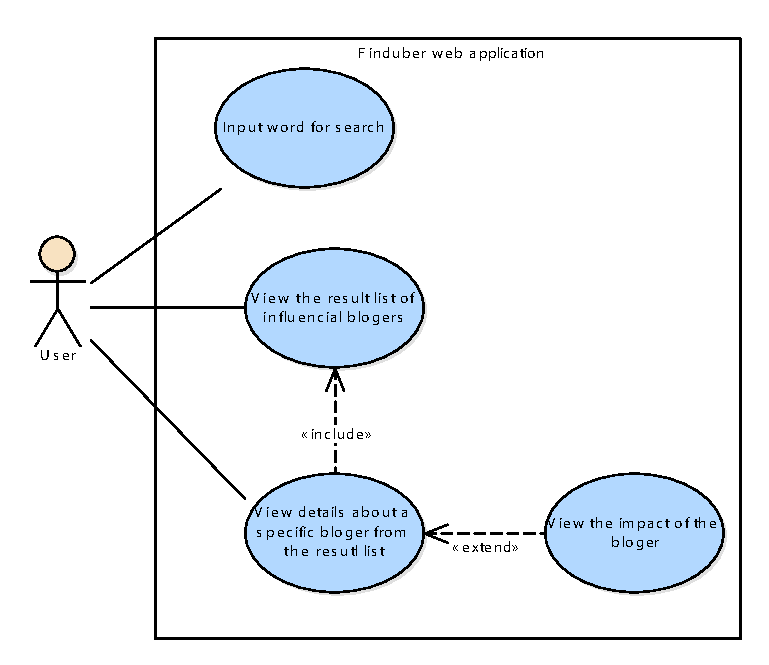
\includegraphics[width=15cm]{UseCase.pdf}
\caption{Use Case Diagram}\label{usecase_uml}
\end{figure}

There are not so many use cases, because the core processes that made the application running where executed in backend. Thus, the user are using only the system functionalities. First use case represents the primary functionality of the system handled by search engine. 

The use case diagrams specify the events of the system and their flows, but never describes how they are implemented. To fulfill this sequence diagrams are used. Moreover, they captures the time sequence of messages flow from one object to another. 

Since it uses objects to show the messages flow and objects are derived from classes, the sequence diagrams are dependent upon class diagrams. Thus, first will be shown the class diagrams and after that the sequence ones. 

\subsection{Class Diagrams}

The class diagrams help us to model and analyse the static views of the application. Through them the responsabilities of the system are described. Each class entity has its own methods and attributes. In the Figure \ref{classCreate_uml} are shown the classes responsabile for database creation. 

\begin{figure}[!ht]
\centering
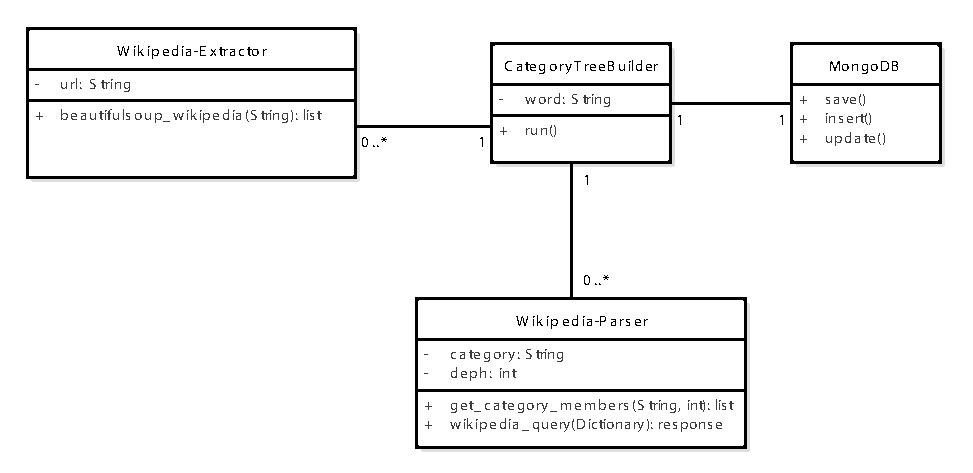
\includegraphics[width=15cm]{create-db}
\caption{Database Creation Class Diagram}\label{classCreate_uml}
\end{figure}

The \textit{CategoryTreeBuilder} class is responsible for setting the order of methods to be called in order to create the database. First the \textit{Wiki\_Extractor} calss is called, which has the responsiblity to extract the web page from the given url. The class \textit{Wikipedia\_Parser} has two attributes and two methods that are working with wikipedia API. Thus, the class is responsible to request particular "actions" by specifying an action parameter, mainly "action=query" to get information.. \textit{MongoDB} class has the task to save the records to database according to the model.  

Structure of database model is shown in Figure \ref{classMongo_uml}

\begin{figure}[!ht]
\centering
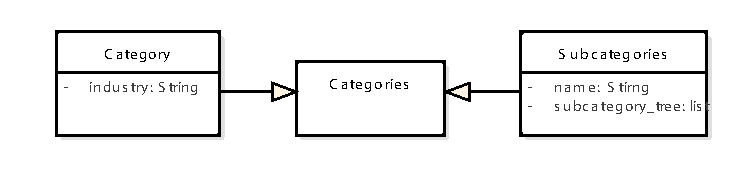
\includegraphics[width=15cm]{MongoDB}
\caption{MongoDB Models Class Diagram}\label{classMongo_uml}
\end{figure}

Although it has a simple structure, the mongodb document is well structured. \textit{Category} holds the industry for which the category tree is composed. \textit{Subcategories} holds an array of embedded documents that contain the fields \textit{name} and \textit{subcategory\_tree}. The subcategory\_tree field is an array of strings. 

A more complex class diagram is build for MapReduce framework used for word frequency count. It has five classes responsible for creating a parallel, distributed algorithm on a cluster for processing large data sets. For Finduber the local machine will act as Server and as Client at the same time. The relations between classes are shown in Figure \ref{hadoop_uml}.

\begin{figure}[!ht]
\centering
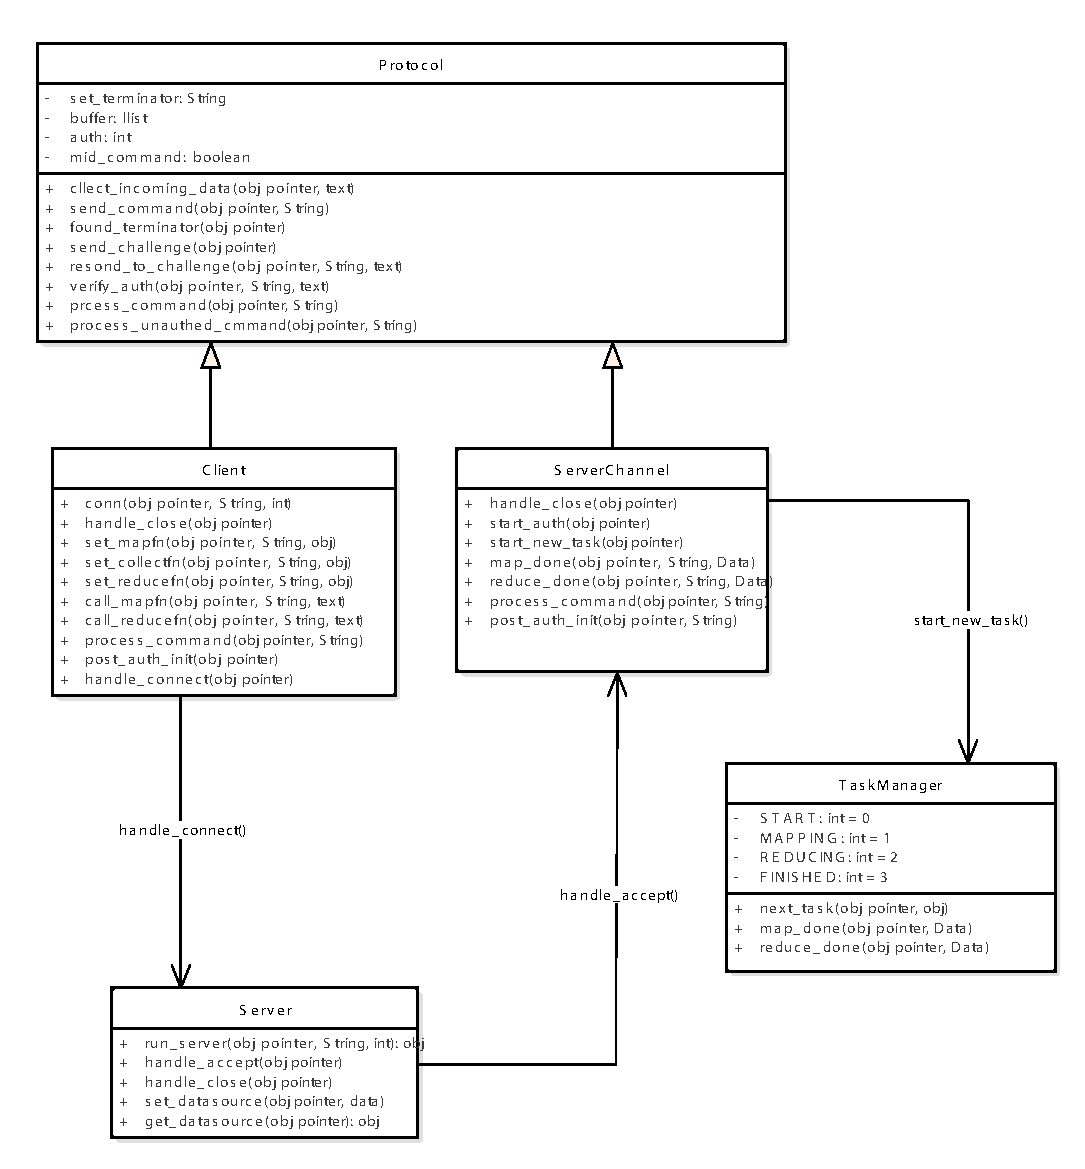
\includegraphics[width=15cm]{hadoop}
\caption{MapReduce Class Diagram}\label{hadoop_uml}
\end{figure}

Now, when all the main classes for Finduber system are documented the sequence diagrams can be created.

\subsection{Sequence Diagrams}

The sequence diagrams are used primarily to show the interactions between objects in the sequential order that those interactions occur. They also can be used as a requirements document to communicate requirements for a future system implementation. Sequence diagrams listed below are only for main processes of the running system at a particular moment. 

In the Figure \ref{createDB_uml} is described the process of creation the categories database. The sequence diagram is having four objects Execute, Wikipedia-Extractor, Wikipedia-Parser and MongoDB, detailed described in Figure \ref{classCreate_uml}.

\begin{figure}[!ht]
\centering
\includegraphics[width=15cm]{CreateDB-1}
\caption{Database Creation Sequence Diagram}\label{createDB_uml}
\end{figure}

The first call is \textit{beautifulsoup\_wikipedia(industry)} wich is a method of \textit{Wikipedia-Extractor} object. The method returns a list of categories for the given industry. The next call is \textit{get\_category\_members (catgeory[1], 1)} which is also a method of \textit{Wikipedia-Extractor} object. To return a response the \textit{Wikipedia-Extractor} object executes a self call \textit{wikipedia\_query}. After this a list of all category members is returned. The returned list is stored in different documents of Mongo database through the call \textit{categories.insert()}.

Since the last return was a list of categories members, the next calls are executed in a loop. The loop control structure is represented in the diagram as a fragmanet with the condition: for all categories. 

First call in the loop is the same method of the object \textit{Wikipedia-Extractor} explained above -- \textit{get\_category\_members(subcategory, 0)} but with different parameters. The last call here is \textit{categories.update()} which is method of \textit{MongoDB} object. It updates the documents of the database with additional inofrmation from the return list. 

The whole proceess of database creation is executed in a loop for all industries that requires a category tree. 

The next sequence diagram shown in Figure \ref{mapreduce_uml} illustrates what is happening in the backend, when user executes a search request.

\begin{figure}[!ht]
\centering
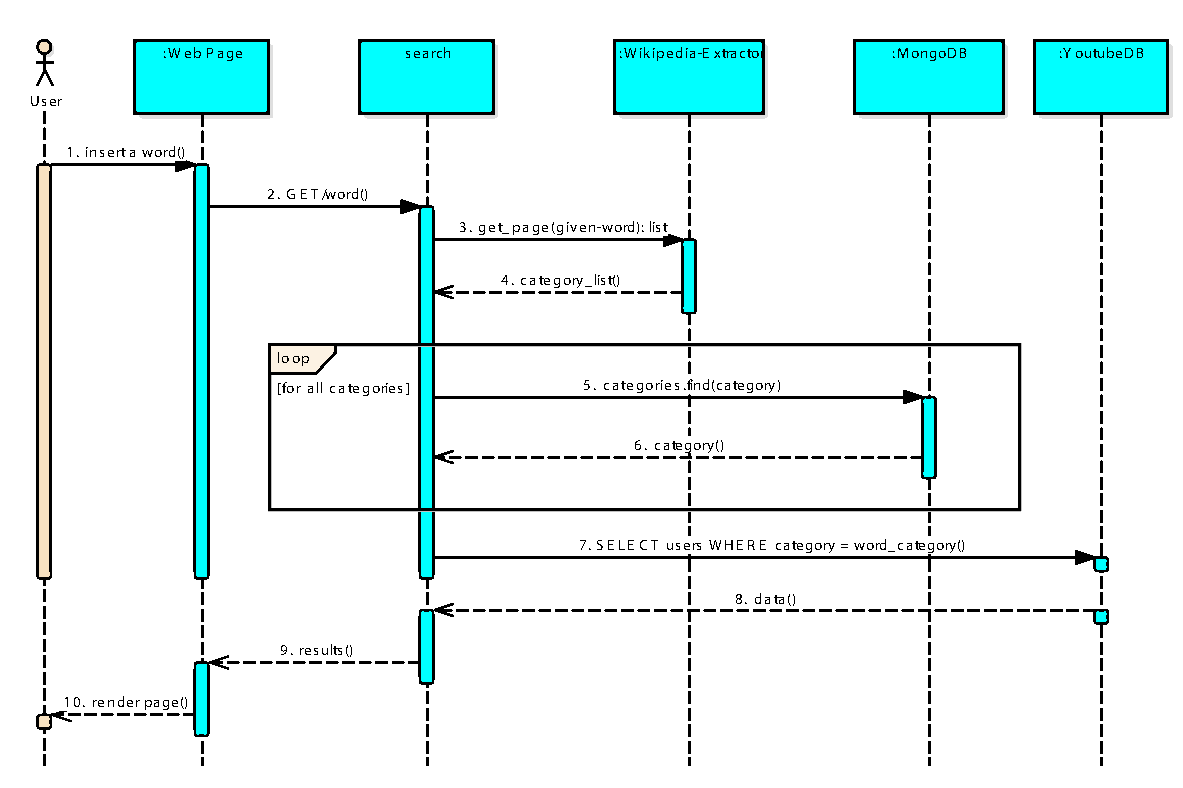
\includegraphics[width=15cm]{SearchDB}
\caption{Database Creation Sequence Diagram}\label{mapreduce_uml}
\end{figure}

First, the search controller gets the user input. The next call is to Wikipedi-Extractor object which is responsable to extract the corresponding wikipedia page and filter the categories. Then, are executed queries to MongoDB in a loop, to find out from to which category the given word belongs. The last call is also a query, but now to PostgreDB, that keep the information about all youtube users with specified categories and other information.

Having the sequnce diagrams it can be easily seen how tasks are distributed between components, also to iddentify patterns of interaction that make it difficult to update the software.

\subsection{Activity Diagram}

Another important diagram that describes the dynamic aspects of the Finduber system is activity diagram. It shows the flow from one activity to another activity. For a better understanding of the described flow swimlanes are used. They group activities performed by the same thread as showm in Figure \ref{doc_uml}. 

\begin{figure}[!ht]
\centering
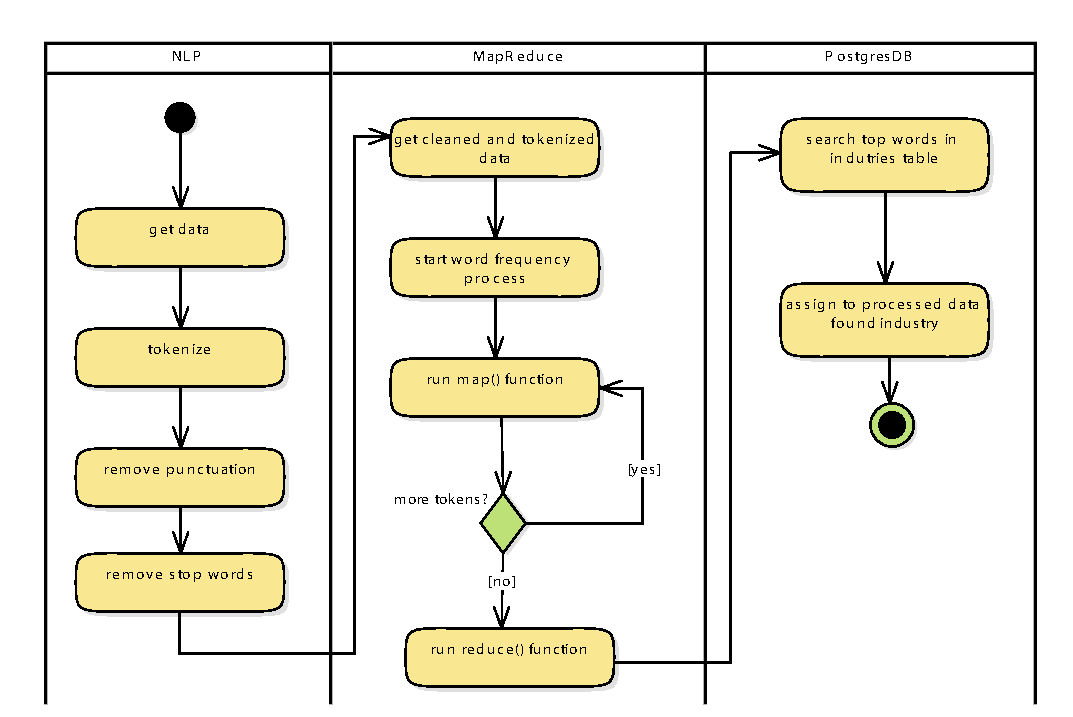
\includegraphics[width=15cm]{MapReduce}
\caption{MapReduce Activity Diagram}\label{doc_uml}
\end{figure}

First swimlane -- NLP -- is responsible for text pre-processing. The process starts when it receives the raw data. Next step is to split it into tokens. Further, from the list of tokens punctuation and insignificant words like: prepositions, conjunctions are removed. To reduce the ammount of tokens and group morphological forms of a word that are assumed to have the same base meaning. When the pre-processing step is done, the activity flow is sent to the MapReduce object. 

MapReduce object gets the cleaned and tokenized data and starts the word frequnecy process. The process consists of functions: Map() that performs filltering and sorting (creates one queue for each word from the text) and Reduce() that executes a summary operations 
(counting the number of words in each queue, yielding frequencies). 

After MapReduce set of activities the data is ready to use in database categorization. Thus, the activity flow goes to PostgresDB object. Its main reponsability is to assign to each record a pre-defined category, based on words with the highest frequency index. 

\subsection{State Machine Diagram}

State diagram is one of the five UML diagrams used to model dynamic nature of a system. They define different states of an object during its lifetime. Statechart diagrams are very important for describing the states. States can be identified as the condition of objects when a particular event occurs. The diagram \ref{state_uml} represents the main state through which the word inputted by user goes. 

\begin{figure}[!ht]
\centering
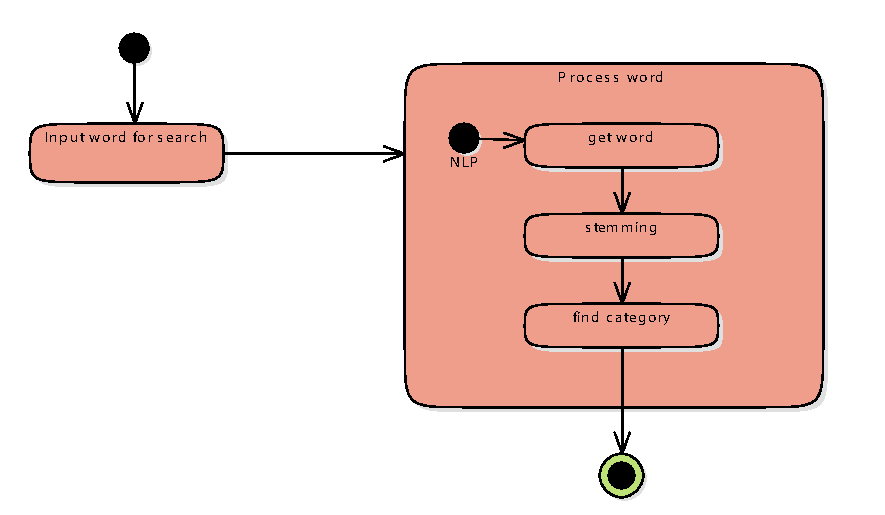
\includegraphics[width=15cm]{wordstate}
\caption{State Diagram}\label{state_uml}
\end{figure}

The first state -- Input word for search -- is an idle state from where the process starts. Next the word get in state of NLP process. The NLP process state has three nested states: get word, stemming, find category. 

Comnning back to the client part of the application, in the Figure \ref{appstates} is shown the application state diagram. Since Finduber proeject do not have so many usecases, there is a few number of states that an user can be in.

\begin{figure}[!ht]
\centering
\includegraphics[width=15cm]{appstate}
\caption{Application State Diagram}\label{appstates}
\end{figure}

As is seen all application states are mapped to a browser page. The entire process starts when the user open the application web page. After that the user is in a state where is able to input words for search. Next states are related to the further possibilities regarding obtained list of results. Three options are available: exit the page without getting in another state, click on a blogger from the list and view details about it and then exit or simply go to the Youtube page of the blogger.

\subsection{Component Diagram}

Another important part of the system architecture is to model physical aspects. In this case, the component diagram is used to shows the structure a software system. By thinking of your system as a collection of components with well-defined provided and required interfaces, you improve the separation between the components. This in turn makes the design easier to understand and easier to change when requirements change.

Component diagram is used to represent the system design regardless of what language or platform the design uses or will use. In the Figure \ref{component_uml} are depicted libraries and frameworks used by Finduber app.
 
\begin{figure}[!ht]
\centering
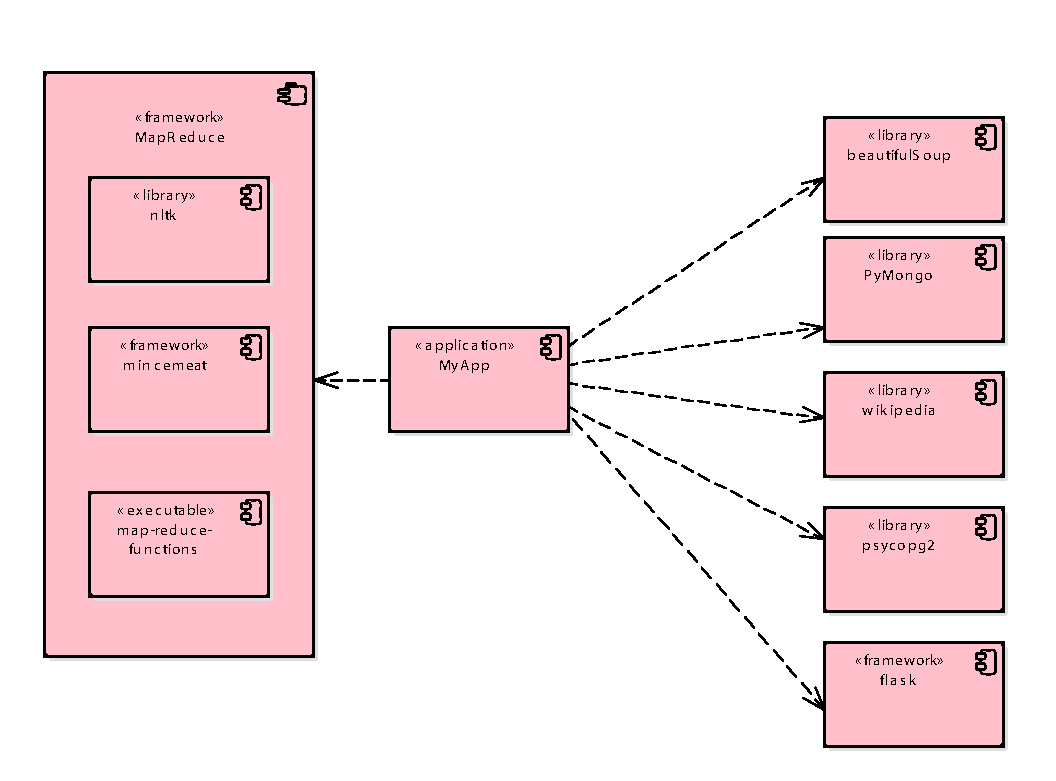
\includegraphics[width=15cm]{Component}
\caption{Component Diagram}\label{component_uml}
\end{figure}

Because the project is devided in two parts there are two sets of libraries. The MapReduce framework is a console application and therefore it uses less libraries. The most important is the mincemeat framework that handle the server-client communication and parallel, distributed algorithm on a cluster. Another usefull library used is nltk. It is a platform that works with human language data that has over 50 corpora and lexical resources, along with a suite of text processing libraries for classification, tokenization and stemming. 

The second set of components are used for user interface application. PyMongo and pscycopg2 deal with database connection and queries. Wikipedia and beautifulSoup libraries are used to pull data out of HTML. 

Figure \ref{component_uml} gives only an overview of existing components, not the topology itself. That is why it is need to create a deployment diagram. 

\subsection{Deployment Diagram}

The Deployment Diagram models the run-time configuration in a static view and visualizes the distribution of components in an application. It involves modeling the hardware configurations together with the software components that lived on.

\begin{figure}[!ht]
\centering
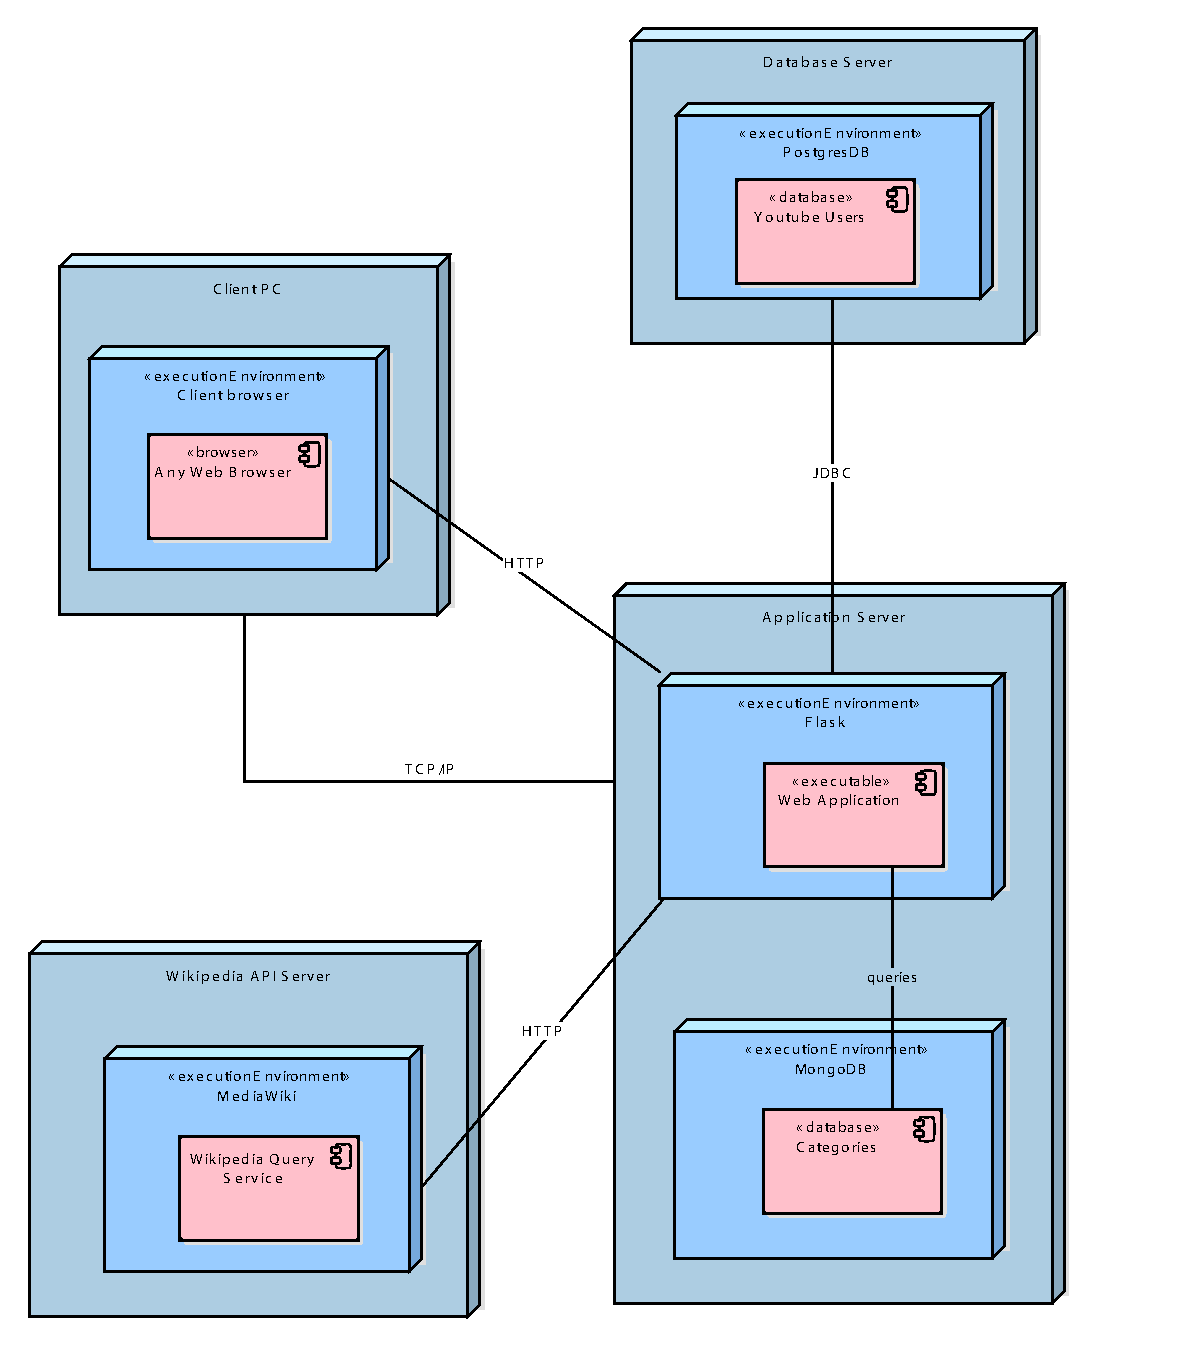
\includegraphics[width=15cm]{Deployment}
\caption{Finduber Deployment Diagram}\label{deploy_uml}
\end{figure}

The system represents a web browser application, thus the execution environment for the client side is a web browser. It connects to application server over HTTP. Application server consists of two environments flask framework and mongodb database. It is also dependent of two others nodes that are outside application server. MediaWiki environment is used for extracting the wikipedia page of the requested word in during execution time and use HTTP to connect to it. Database server holds youtube users database and the connection to it is made over JDBC.









 






